\chapter{Europe rail networks - Task 45}

A comprehensive dataset of European railroads (2019) from \href{https://www.mapsforeurope.org/datasets/euro-global-map}{EuroGlobalMap} is analyzed. 
The dataset consists of two objects: linestrings\footnote{Linestring objects are a series of points (each with its own coordinate) connected successively with each other.} and points, the former represent rail roads, while the latter are train stations. 
The resulting graph consists of two kind of nodes, station ($s$) and non-station ($ns$) nodes.\\
Although the fine details can be very important, the first instinct was to use the $ns$ nodes to build a network consisting entirely of $s$ nodes, connected if a path that does not cross any other $s$ node exists between them. However, this task is extremely challenging while keeping an undirected graph with no additional node-metadata, the fundamental reason is because of rail junctions.

\begin{wrapfigure}{r}{7.5cm}  
\label{fig:junctionexample}
  \centering
  \vspace{-\baselineskip}    % (optional) nudge upward a bit
  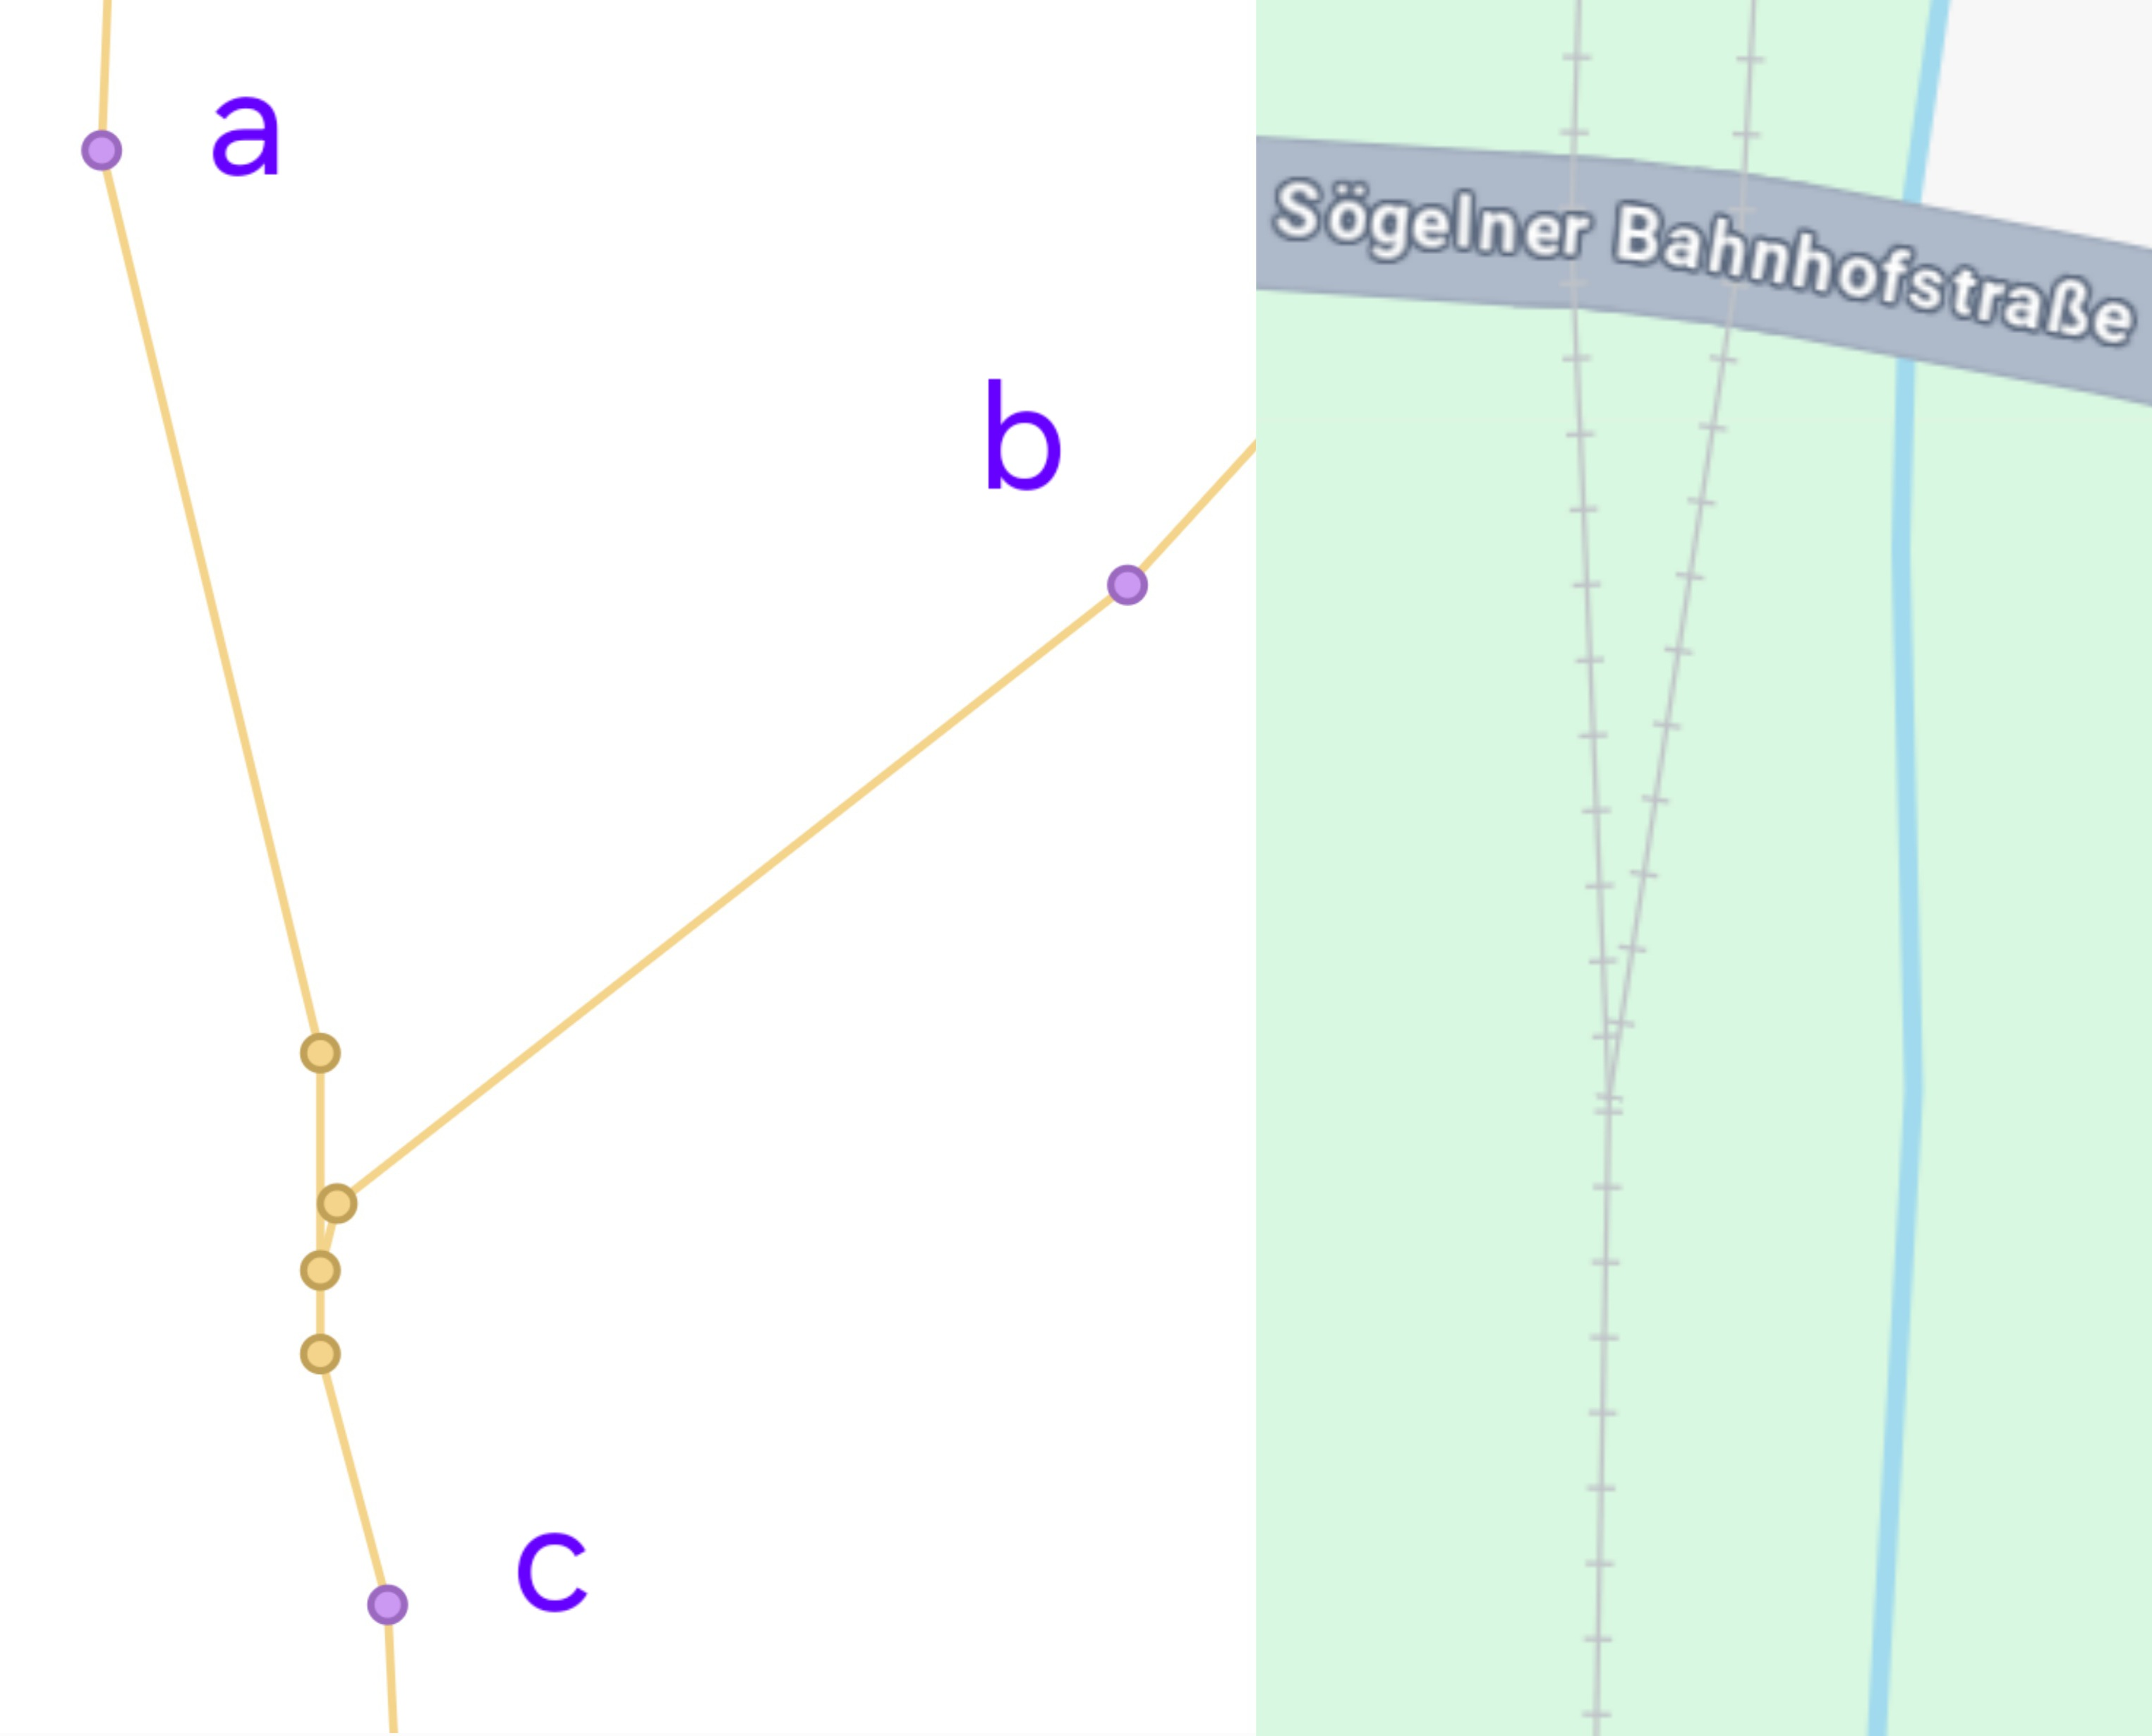
\includegraphics[width=\linewidth,keepaspectratio]{images/junction_example.jpg}
  \caption{German rail junction. a, b and c are $s$ nodes; on the right a Maps view.}

\end{wrapfigure}
In the provided example, it is clear that in order to go from $a$ to $b$, one must pass through $c$, and, while in this case the connection is straightforward ($a \, - \, c$  ;  $b\, - \, c$) a lot of junctions are intertwined with each other and there are many edge cases.\\
Until the definition of \emph{path} is addressed properly, centrality measures of betweenness and closeness could be misleading.

The objective is therefore to prune the network as much as possible, using only non-spatial topological features, such as degree, while retaining all the useful information on how different stations are connected with each other\footnote{Note that in the pruning process, one could keep records of the distance between $ns$ nodes before removing them, and encode it in the edges of the pruned graph.}.
\\
\\
\\
\\
\\
\\
\section{Data description}
Linestring objects are an approximation of the rail track as a series of segments, the ends of those segments are the $ns$ nodes, each with its coordinate.\\
Points in in the rail station data represent train stations, those are the $s$ nodes.\\
All of the $s$ nodes' coordinates are present in the rail dataset, and they match exactly, in particular, they are always found to be at the beginning or at the end of a linesting.\\

Coordinate pairs are expressed in EPSG 4258 (ETRS89) CRS notation, their precision
varies from pinpoint to about $500 \, \,m$, but given the exact matching between the two datasets, this is not a problem.\\
Each station carries a Transport Facility Type (TFC) code, which distinguishes passenger-facing stops (stations, halts, joint stations) from freight-oriented facilities (marshalling yards and intermodal terminals) or maintenance depots. By filtering on TFC it is possible to extract a pure passenger network, isolate cargo terminals, or even build a graph of just the utility lines used for yard operations.
For some countries the TFC is not provided, and it defaults to $0$, those are Croatia, Moldova, Norway, Ukraine, Bulgaria ($88\%$), Luxembourg($14\%$), and Latvia($12\%$).\\

Note that not all the stations are present: section \ref{app:missing} compares, for each country, the number of stations available in the dataset against publicly reported figures. While these reference counts aren’t exact, they provide a useful order-of-magnitude estimate of dataset coverage by country.

The resulting graph object is constructed using the rail data, promoting a $ns$ node to $s$ node if its coordinates appear in the station dataset.
\begin{figure}[htbp]
  \centering
  \includegraphics[width=10.5cm,keepaspectratio]{images/Spain_and_Portugal.png}
  \caption{Rail network of Spain and Portugal, $s$ nodes in purple.}

\end{figure}

\section{Pruning algorithm, overview and visualization}
Upon data extraction, each linestring object is immediately reduced to just the first, second, second-last, and last points; then, a list of protected nodes is defined, its elements are: $s$ nodes, neighbors of nodes $v$ s.t. $k_v \geq 3$ and $v$ does not belong in any $3-clique$, all nodes that belong in a $3-clique$.\\
The choice of protecting neighbors of high-degree nodes is an attempt to preserve the spatial information that would be needed to decide which paths are allowed through a junction\footnote{this can be achieved by forbidding the path between the nodes that form the lowest angle with that junction (although it is not that easy for 3 or 4 way junctions)}. The focus on 3-cliques is motivated by the fact that those types of junction always connect everyone with everyone else, without needing spatial information.\\
The algorithm itself first removes non protected degree-1 (dangling) nodes, than all non protected degree-2 nodes, then, possible 3-cliques are detected and formed. \\

\begin{figure}[htbp]
  \centering
  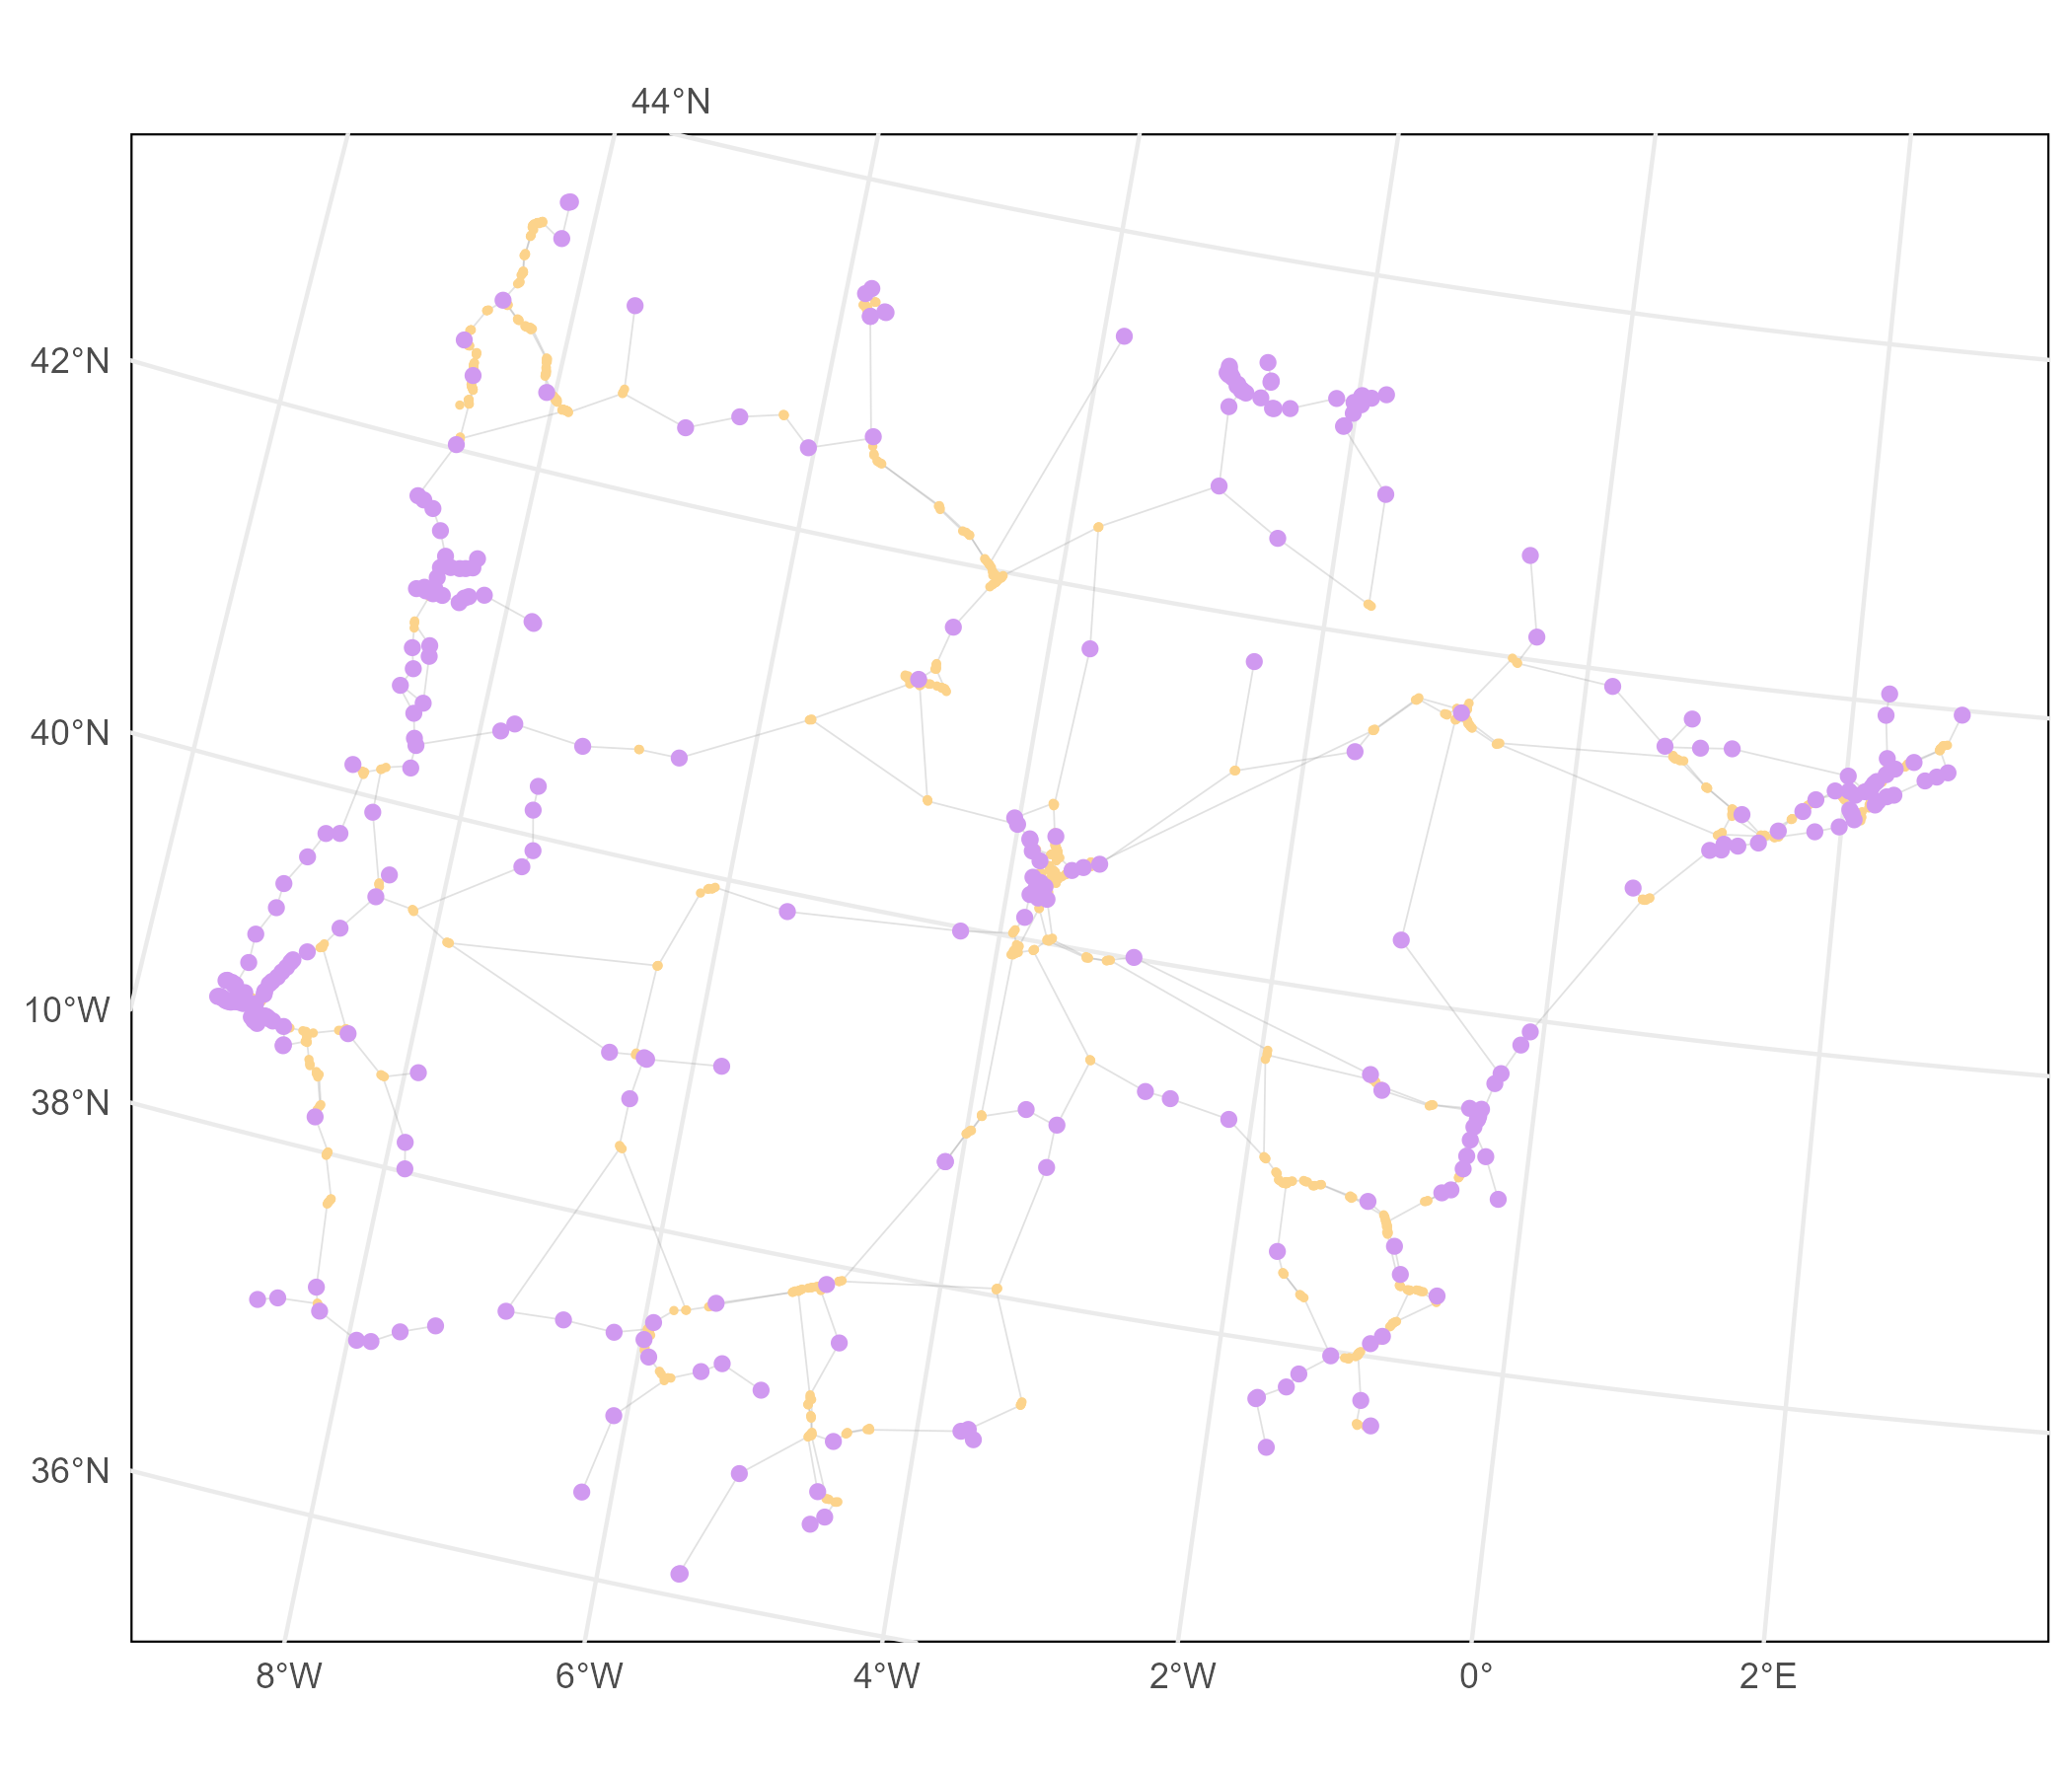
\includegraphics[width=10.5cm,keepaspectratio]{images/Spain_and_portugal_pruned.png}
  \caption{Pruned rail network of Spain and Portugal, $s$ nodes in purple.}

\end{figure}

Throughout the process, an interactive visualization tool was used; here is a 
\href{https://ale-neri-137.github.io/PoCN_project/french_rail_before.html}{before} and 
\href{https://ale-neri-137.github.io/PoCN_project/french_rail_after.html}{after} example for the French rail network. See appendix \ref{app:ralvis}, for additional figures.

 




\newpage
